\section{Einleitung}
In diesem Versuch geht es um die spektrale Zerlegung verschiedener Lichtquellen. Anhand des Spektrums können Aussagen über die Lichtquellen gemacht werden.
Bei einem Spektrometer wird zunächst mit Hilfe einer Linse ein paralleles Lichtbündel hergestellt. Dieses wird durch ein Prisma aufgrund der Wellenlängenabhängigkeit des Brechungsindexes in die verschiedenen Wellenlängen aufgeteilt. Diese Lichtstrahlen gehen durch eine zweite Linse und werden nach Wellenlängen auf einen Schirm fokussiert.
Anstelle eines Prismas ist es auch möglich ein Spektrometer mit einem Beugungsgitter zu realisieren. Dieses hat einen Vorteil bei der Bestimmung der Wellenlänge. Diese kann durch das Abzählen der Beugungsordnung $ \textit{m} $ und anhand der Winkels der zugehörigen Beugungswinkel $ \vartheta_{m} $ zusammen mit der Gitterkonstanten $ \textit{g} $ folgt für die Wellenlänge,
\begin{equation}
\lambda=\frac{g\cdot\sin \vartheta_{m}}{m} \label{Wellenlänge}
\end{equation}
daraus lassen sich für unterschiedliche Lichtquellen charakteristische Spektren bestimmen ( zum Beispiel das Linienspektrum einer Natrium-Dampflampe). 
Eine Eigenschaft die zu berücksichtigen ist, ist das Auflösungsvermögen des Spektrometers.
Also wie groß der Wellenlängenunterschied $ \triangle\lambda $ sein muss, damit zwei Linien klar unterscheidbar sind.
Das Auflösungsvermögen $ \textit{A} $ ist definiert als,
\begin{equation}
A=\frac{\lambda}{\triangle\lambda_{min}}
\end{equation}
hierbei ist $ \triangle\lambda_{min} $ die noch kleinste trennbare Wellenlängendifferenz zweier Linien ist und $ \lambda $ die mittlere Wellenlänge der Linien.
Das Rayleigh-Kriterium für das Auflösungsvermögen lautet,
\begin{equation}
\frac{\lambda}{\triangle\lambda_{min}}=mN
\end{equation}
hierbei ist $ \textit{m} $ die Beugungsordnung und  $ \textit{N} $ die Anzahl der beleuchteten Spalte.
In diesem Versuch werden unter anderem die Linienspektren von Gasen untersucht.
Gase emittieren nur diskrete Spektren, da die Elektronen nur auf bestimmten Energieniveaus sein können. Werden die Elektronen des Gases angeregt (durch Hitze oder elektrischer Spannung) können diese nur auf diskrete Niveaus höherer Energie angehoben werden. Dieser Zustand ist allerdings nicht stabil, also "fällt" das Elektron wieder auf sein ursprüngliches Energieniveau zurück. Dabei kann es die überschüssige Energie in Form von Licht abgeben, dabei folgt es der Gleichung
\begin{equation}
\lambda=\frac{hc}{\triangle E}
\end{equation}
$ \triangle E $ ist die Energiedifferenz zwischen Anfangs- und Endzustand, $ \textit{h} $ ist das Planksche Wirkungsquantum, $ \textit{c} $ ist die Lichtgeschwindigkeit und $ \lambda $ die Wellenlänge des emittierten Lichts. 
Dadurch lassen sich beispielsweise Rückschlüsse auf die Zusammensetzung des Füllgases einer Energiesparlampe schließen.
Bei Leuchtdioden sind die Spektren nicht diskret, sonder sie überdecken kontinuierlich ganze Energiebereiche. Diese werden Energiebänder genannt. 
Eine Leuchtdiode emittiert Licht, wenn die Elektronen des p-dotierten Substrates sich durch Anregung (elektrische Spannung) mit den "Löchern" des n-dotierten Substrates rekombinieren. Die emittierten Wellenlängen verteilen sich kontinuierlich über das Gesamte Energieband. Es gilt,
\begin{equation}
\lambda=\frac{hc}{E_{G}}
\end{equation}
$ E_{G} $ liegt bei Halbleitern bei etwa 1-3 eV.

\newpage
\section{Auswertung}
\subsection{Prisma und Gitter}
Wird das Prisma als optische Komponente im Spektrometer verwendet und so ausgerichtet, dass der Strahlengang symmetrisch ist. Der Spalt wird mit einer  Natriumdampflampe ausgeleuchtet. Es sind wie erwartet zwei Linien sichtbar. Diese Linien waren aber nicht gerade sondern leicht gekrümmt, was auf eine nicht ganz richtige Ausrichtung des Spektrometers zurückzuführen ist.
Wird das Prisma durch das Transmissionsgitter mit $ g=\SI{1/300}{\milli\meter} $  ersetzt, sind Linien bis zur 4 Beugungsordnung auffindbar. Dabei ist auffällig, dass je höher die Beugungsordnung wird, desto mehr war erkennbar, dass es sich um zwei sich überschneidende Linien handelt. Diese sind nicht scharf unterscheidbar.
\begin{tabular}{|c|c|c|}
\hline 
Beugungsordnung & Lage der Hauptmaxima links & Lage der Hauptmaxima rechts \\ 
\hline 
0 & 0 & 0 \\ 
\hline 
1 & 10 & 349,75 \\ 
\hline 
2 & 20,5 & 339,5 \\ 
\hline 
3 & 31,75 & 328,25 \\ 
\hline 
4 & 44,5 & 315,25 \\ 
\hline 
\end{tabular} 
Die Fehler für die Gradzahlen betragen $ \pm 0,25 $.
Wird das Transmissuinsgitter mit einem ausgetauscht, dessen Gitterkonstante $ g=\SI{1/600}{\milli\meter} $ so ist zu beobachten, dass die Hauptmaxima weiter auseinander gehen ( Abstände verdoppeln sich) und das die Intensität stärker abnimmt.


\subsection{Heliumdampflampe}
Um die abgelesenen Winkel des Spektrums in Wellenlängen zu übertragen, wird anhand des Spektrums einer Heliumlampe folgende Grafik erstellt,
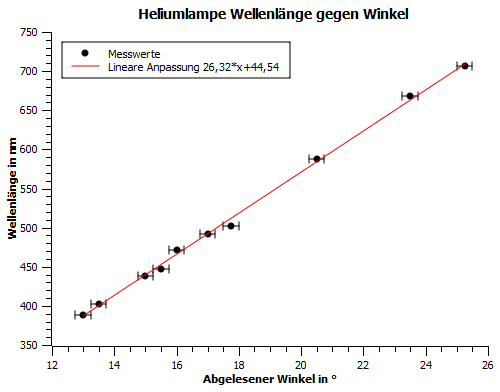
\includegraphics[scale=1]{../../Documents/GitHub/Praktikum-SS15/praktikum/O3/Heliumlampe_Grafik.png} 
somit erhöht sich die Wellenlänge um $ \SI{26,32}{\nano\meter} $ pro Grad.

\newpage
\section{Diskussion}
\subsection{Auflösungsvermögen}
Vergleicht man die Spektren der verschiedenen dispergierenden Elemente, so ist der auffälligste Unterschied, dass beim Prisma zwei scharf trennbare Linien sichtbar sind. Bei den Gittern sind mit zunehmender Beugungsordnung zwei sich überschneidende Linien zu erkennen, daraus ist zu schließen, dass der Wellenlängenunterschied zu gering ist, um scharfe Linien aufzulösen.
Dieser beträgt bei der verwendeten Natriumdampflampe $ \SI{0,6}{\nano\meter} $. Die Gitter unterscheiden sich durch ihre Spaltenanzahl, daraus ergibt sich wie nach dem Rayleigh-Kriterium eine bessere Unterscheitbarkeit der sich überschneidenden Linien. 
